\documentclass[12pt,a4paper]{article}
\usepackage[utf8]{inputenc}
\usepackage[onehalfspacing]{setspace}
\usepackage[lmargin=3cm,tmargin=3cm,rmargin=2cm,bmargin=2cm]{geometry}
\usepackage[brazil]{babel}
\usepackage[T1]{fontenc}
\usepackage{fancyhdr}
\usepackage{graphicx}
\usepackage{indentfirst}
\usepackage{comment}
\usepackage{enumerate}
\usepackage{listingsutf8}
\usepackage{xcolor}
\usepackage{pgffor}

\definecolor{dkgreen}{rgb}{0,0.6,0}
\definecolor{gray}{rgb}{0.5,0.5,0.5}
\definecolor{mauve}{rgb}{0.58,0,0.82}

\usepackage{hyperref}
\hypersetup{
    colorlinks=true,
    linkcolor=blue,
    filecolor=magenta,
    urlcolor=cyan,
}


\lstset{frame=tb,
  language=C,
  aboveskip=3mm,
  belowskip=3mm,
  showstringspaces=false,
  columns=flexible,
  basicstyle={\small\ttfamily},
  numbers=none,
  numberstyle=\tiny\color{gray},
  keywordstyle=\color{blue},
  commentstyle=\color{dkgreen},
  stringstyle=\color{mauve},
  breaklines=true,
  breakatwhitespace=true,
  tabsize=8,
  extendedchars=true,
  inputencoding=utf8,
  texcl=true,
}
\lstset{literate=%
{í}{{\'i}}1
{ó}{{\'o}}1
{ú}{{\'u}}1
{é}{{\'e}}1
{ê}{{\^e}}1
{á}{{\'a}}1
{ã}{{\~a}}1
{õ}{{\~o}}1
{ô}{{\^o}}1
{ç}{{\c c}}1
}

% numeracao header
\pagestyle{headings}

% quebra de pagina por secao
\let\oldsection\section
\renewcommand\section{\clearpage\oldsection}


\begin{document}

\begin{titlepage}
	\begin{center}
		\textbf{UNIVERSIDADE DE RIBEIRÃO PRETO} \\
			CIÊNCIAS EXATAS \\
			Laboratório de Programação I

			\vspace{1.5cm}

			\textbf{Prof. Rodrigo de Oliveira Plotze}

			\vspace{0.5cm}

			\textbf{Murilo da Silva Ijanc'} \\
			RA: 834125

			\vspace{6.5cm}

			\textbf{ATIVIDADE PARCIAL}

			\vfill

			\vspace{0.8cm}

			
\includegraphics[width=0.2\textwidth]{unaerp}

			\textbf{RIBEIRÃO PRETO} \\
			\textbf{2020}
	\end{center}
\end{titlepage}

\thispagestyle{empty}
\tableofcontents

\newpage
\thispagestyle{empty}

\listoffigures
\newpage

\pagenumbering{arabic}

\section{Introdução}
Abaixo encontram-se as soluções dos exercícios da prova parcial da matéria
de \textbf{Laboratório de Programação I} do primeiro semestre de Engenharia
de Software da Universidade de Ribeirão Preto, a matéria é ministrada pelo
Prof. Rodrigo de Oliveira Plotze.

Os códigos foram escritos no sistema operacional
\href{https://www.openbsd.org}{OpenBSD}, portanto não foi necessário o uso
da biblioteca \textbf{locale.h}, caso utilize um sistema operacional diferente,
provavelmente seja necessário usá-la. Os códigos possuem compatibilidade com os 
compiladores \href{https://gcc.gnu.org/}{GCC-8.3.0} e 
\href{https://clang.llvm.org/}{Clang-8.0.1} e o código fonte pode ser obtido no
repositório \url{https://github.com/murilobsd/lab\_prog\_1}

Os códigos obedecem ao guia de formatação do kernel do OpenBSD que pode ser 
visualizado em \href{https://man.openbsd.org/style}{style(9)}. A licença usada
para os códigos é \href{https://opensource.org/licenses/BSD-3-Clause}{BSD3}

\subsection{Baixando Código Fonte}
\noindent O código pode ser clonado via repositório git ou baixar o
\href{https://github.com/murilobsd/lab_prog_1/archive/0.0.1.zip}{arquivo.zip}

\begin{lstlisting}[language=bash]
  $ git clone https://github.com/murilobsd/lab_prog_1
\end{lstlisting}

\subsection{Compilando}
\noindent No repositório é dispobilizado o arquivo \textbf{Makefile} que deve
ser usado pelo \href{https://www.gnu.org/software/make/}{GNU Make}, como
mostrado abaixo:
\begin{lstlisting}[language=bash]
  $ make all
  compilando exercicio 2: bex1
  cc -O2 -pipe  -Wall -Wextra -Werror -std=c89 -O2 -g ex1.c -o bex1
  compilando exercicio 2: bex2
  cc -O2 -pipe  -Wall -Wextra -Werror -std=c89 -O2 -g ex2.c -o bex2
  compilando exercicio 3: bex3
  ...
\end{lstlisting}

\noindent Ou via linha de comando, abaixo compilando o ex1 (exercício 1):
\begin{lstlisting}[language=bash]
  $ cc -O2 -pipe  -Wall -Wextra -Werror -std=c89 -O2 -g ex1.c -o bex1
\end{lstlisting}

\pagebreak

\section{Exercício 1}
\lstinputlisting{ex1.c}
\begin{figure}[htb!]
	\centering
	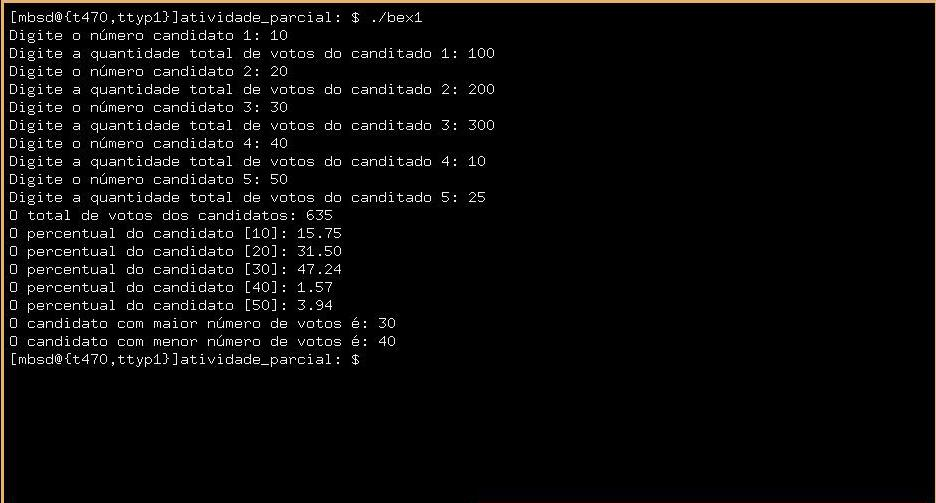
\includegraphics[width=16cm]{ex1}
	\caption{Saída Exercício 1}
	\label{fig:1}
\end{figure}

\section{Exercício 2}
\lstinputlisting{ex2.c}
\begin{figure}[htb!]
	\centering
	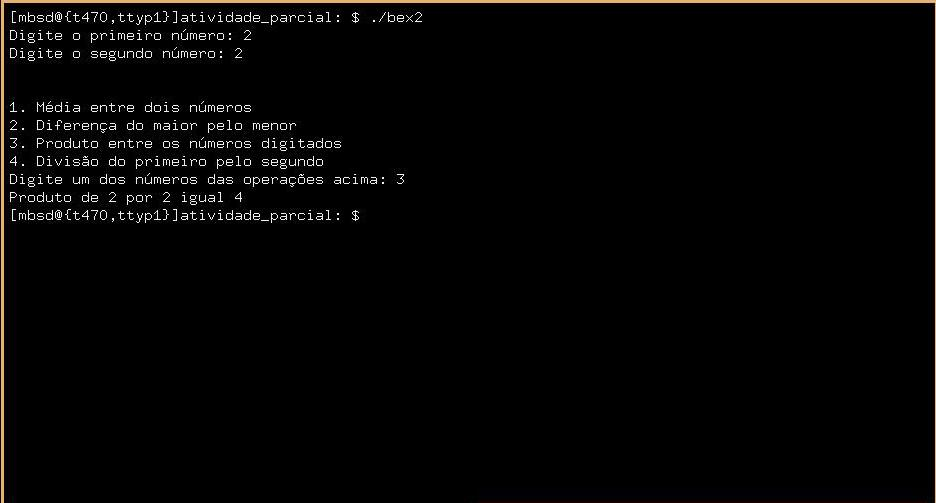
\includegraphics[width=16cm]{ex2}
	\caption{Saída Exercício 2}
	\label{fig:2}
\end{figure}

\section{Exercício 3}
\lstinputlisting{ex3.c}
\begin{figure}[htb!]
	\centering
	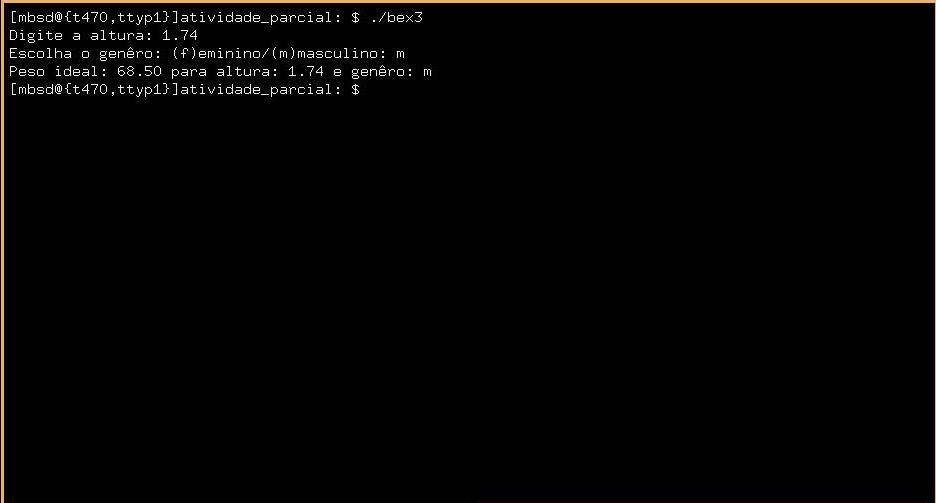
\includegraphics[width=16cm]{ex3}
	\caption{Saída Exercício 3}
	\label{fig:3}
\end{figure}

\section{Exercício 4}
\lstinputlisting{ex4.c}
\begin{figure}[htb!]
	\centering
	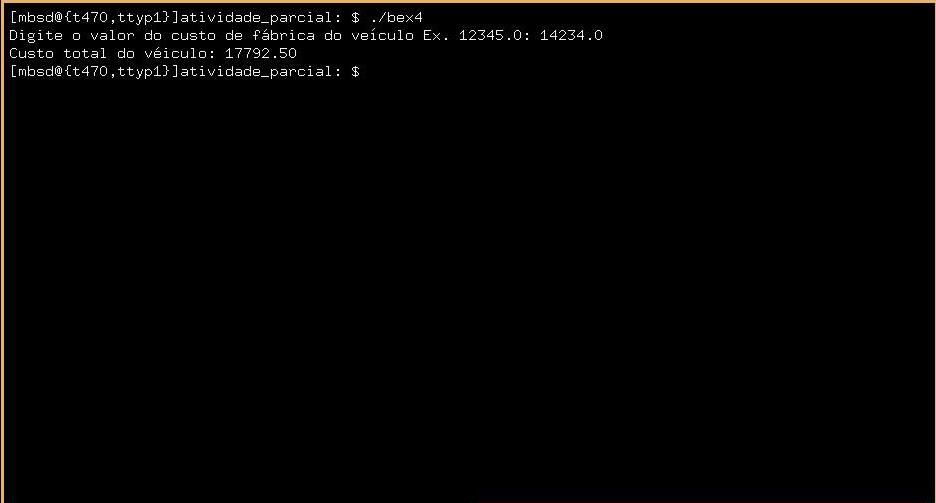
\includegraphics[width=16cm]{ex4}
	\caption{Saída Exercício 4}
	\label{fig:4}
\end{figure}

\section{Exercício 5}
\lstinputlisting{ex5.c}
\begin{figure}[htb!]
	\centering
	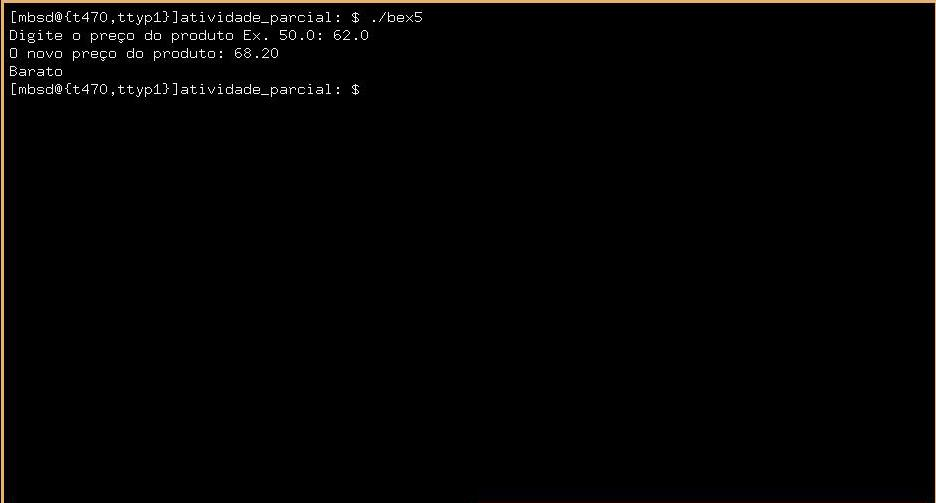
\includegraphics[width=16cm]{ex5}
	\caption{Saída Exercício 5}
	\label{fig:5}
\end{figure}

\section{Exercício 6}
\lstinputlisting{ex6.c}
\begin{figure}[htb!]
	\centering
	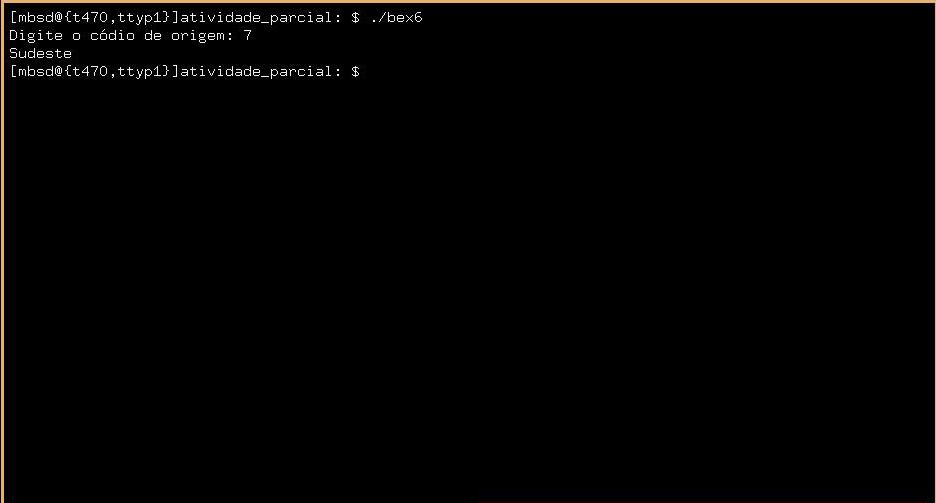
\includegraphics[width=16cm]{ex6}
	\caption{Saída Exercício 6}
	\label{fig:6}
\end{figure}

\section{Exercício 7}
\lstinputlisting{ex7.c}
\begin{figure}[htb!]
	\centering
	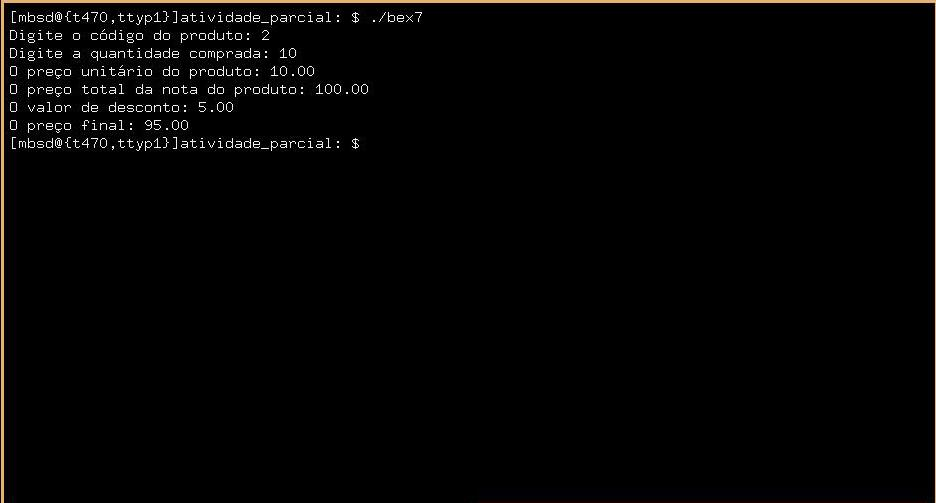
\includegraphics[width=16cm]{ex7}
	\caption{Saída Exercício 7}
	\label{fig:7}
\end{figure}

\section{Exercício 8}
\lstinputlisting{ex8.c}
\begin{figure}[htb!]
	\centering
	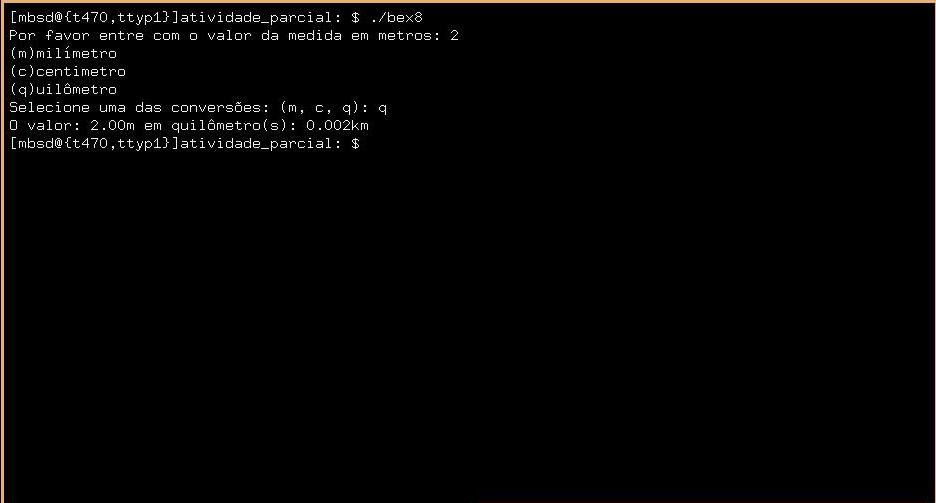
\includegraphics[width=16cm]{ex8}
	\caption{Saída Exercício 8}
	\label{fig:8}
\end{figure}

\section{Exercício 9}
\lstinputlisting{ex9.c}
\begin{figure}[htb!]
	\centering
	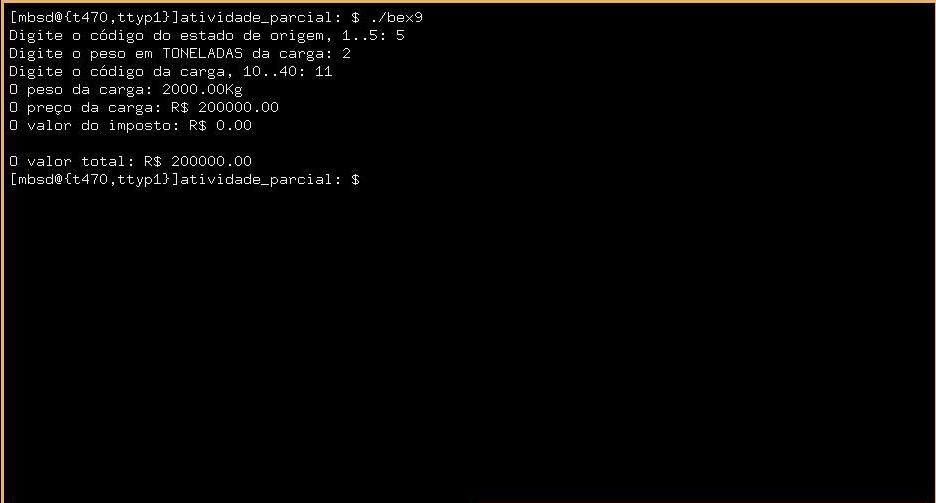
\includegraphics[width=16cm]{ex9}
	\caption{Saída Exercício 9}
	\label{fig:9}
\end{figure}

\section{Exercício 10}
\lstinputlisting{ex10.c}
\begin{figure}[htb!]
	\centering
	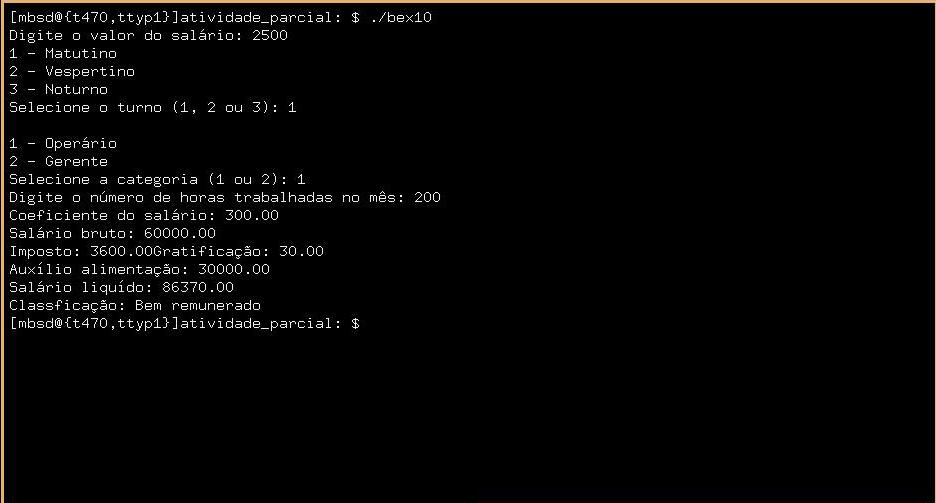
\includegraphics[width=16cm]{ex10}
	\caption{Saída Exercício 10}
	\label{fig:10}
\end{figure}

\end{document}
